\section{User Interface}
A meeting was established with two of the customers, Drazenko and Pernille \citep{misc:drazenko, misc:pernille}.
From the meeting it was found that the general drawing interface seemed suitable, however, after they tried to use the application, some flaws were found.
The flaws were mainly the way to take photos, which was deemed unintuitive, as you had to take multiple pictures and then later choose which one to load into the pictogram.
Furthermore, a new position ordering of the drawing tools was requested.
This was mainly a request from Pernille, as she found that options for the drawing tools should be located near each other.
Additionally, the colour theme of the application was changed such that the graphical components developed by the \textit{GIRAF Components} group was used.

The implemented version can be seen in \appref{app:further-deflopment}

\subsection{Prototypes}
Before the user interface (UI) changes are performed in the application, paper prototypes are created to get a first intuition of how the UI should look.
These prototypes are based upon the talk with the customers \citep{misc:drazenko, misc:pernille}.
 
\subsubsection*{Rearrange UI Components}
Based on the request from the customers, the UI components of the drawing surface should be rearranged.
Two prototypes were drawn for this, which can be seen in \figref{fig:v1drawfrag} and \figref{fig:v2drawfrag}.
The idea of \figref{fig:v1drawfrag} was to move the components that had to do with the creation of a pictogram down in the \textit{drawFragment}. Furthermore, to arrange the options for the drawing tools near the tools themselves.
However, it was deemed that the application became asymmetrical due to this change.

\begin{figure}[h]
     \centering
     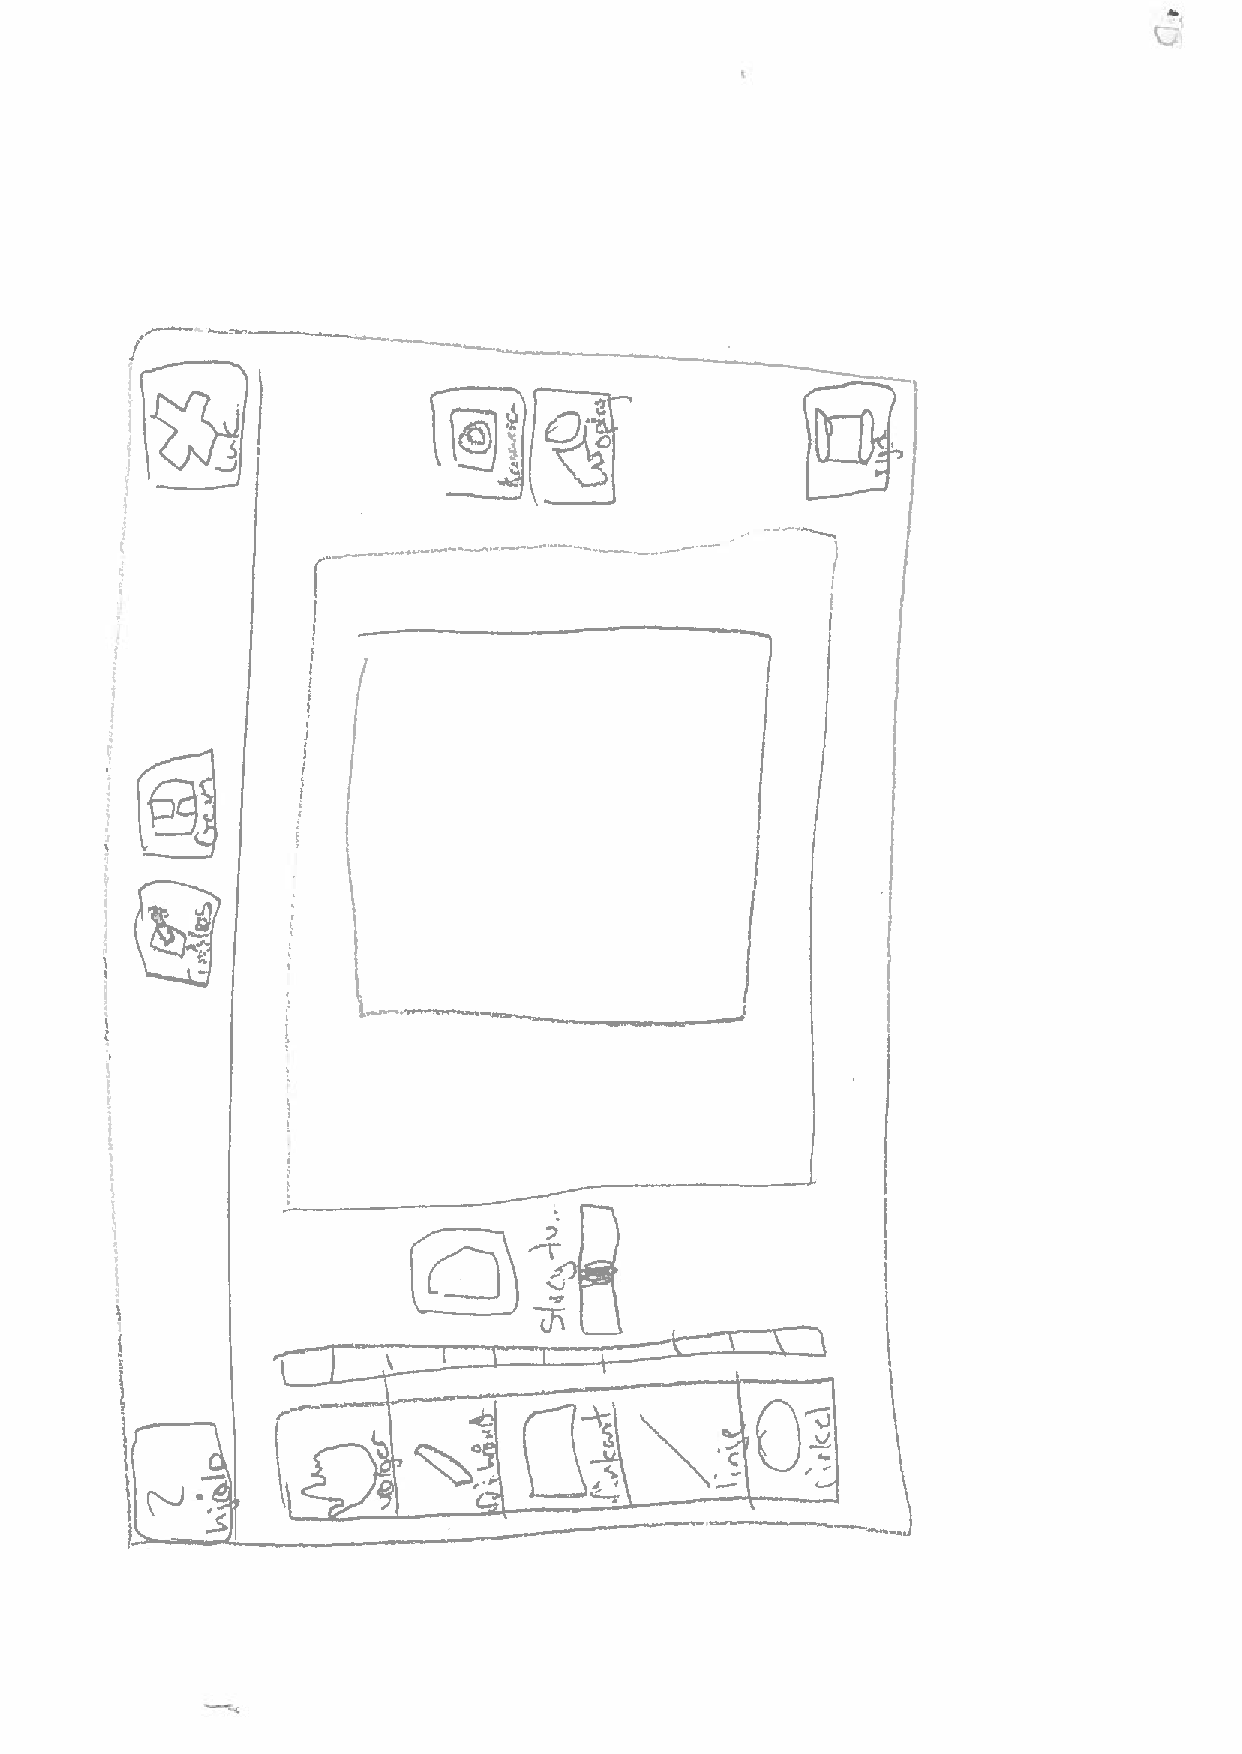
\includegraphics[angle=270, scale=0.5, trim = 1.5cm 3cm 5.5cm 5.5cm,clip]{sprint3/v1-drawfragment.pdf}
     \caption{Version 1 drawfragment.}
     \label{fig:v1drawfrag}
\end{figure}

The idea of \figref{fig:v2drawfrag} was to keep everything drawing related in the \textit{drawFragment} and additional features in the top bar. In addition, the options of the drawing tools were separated from the tools themselves, to regain symmetry.

\begin{figure}[h]
     \centering
     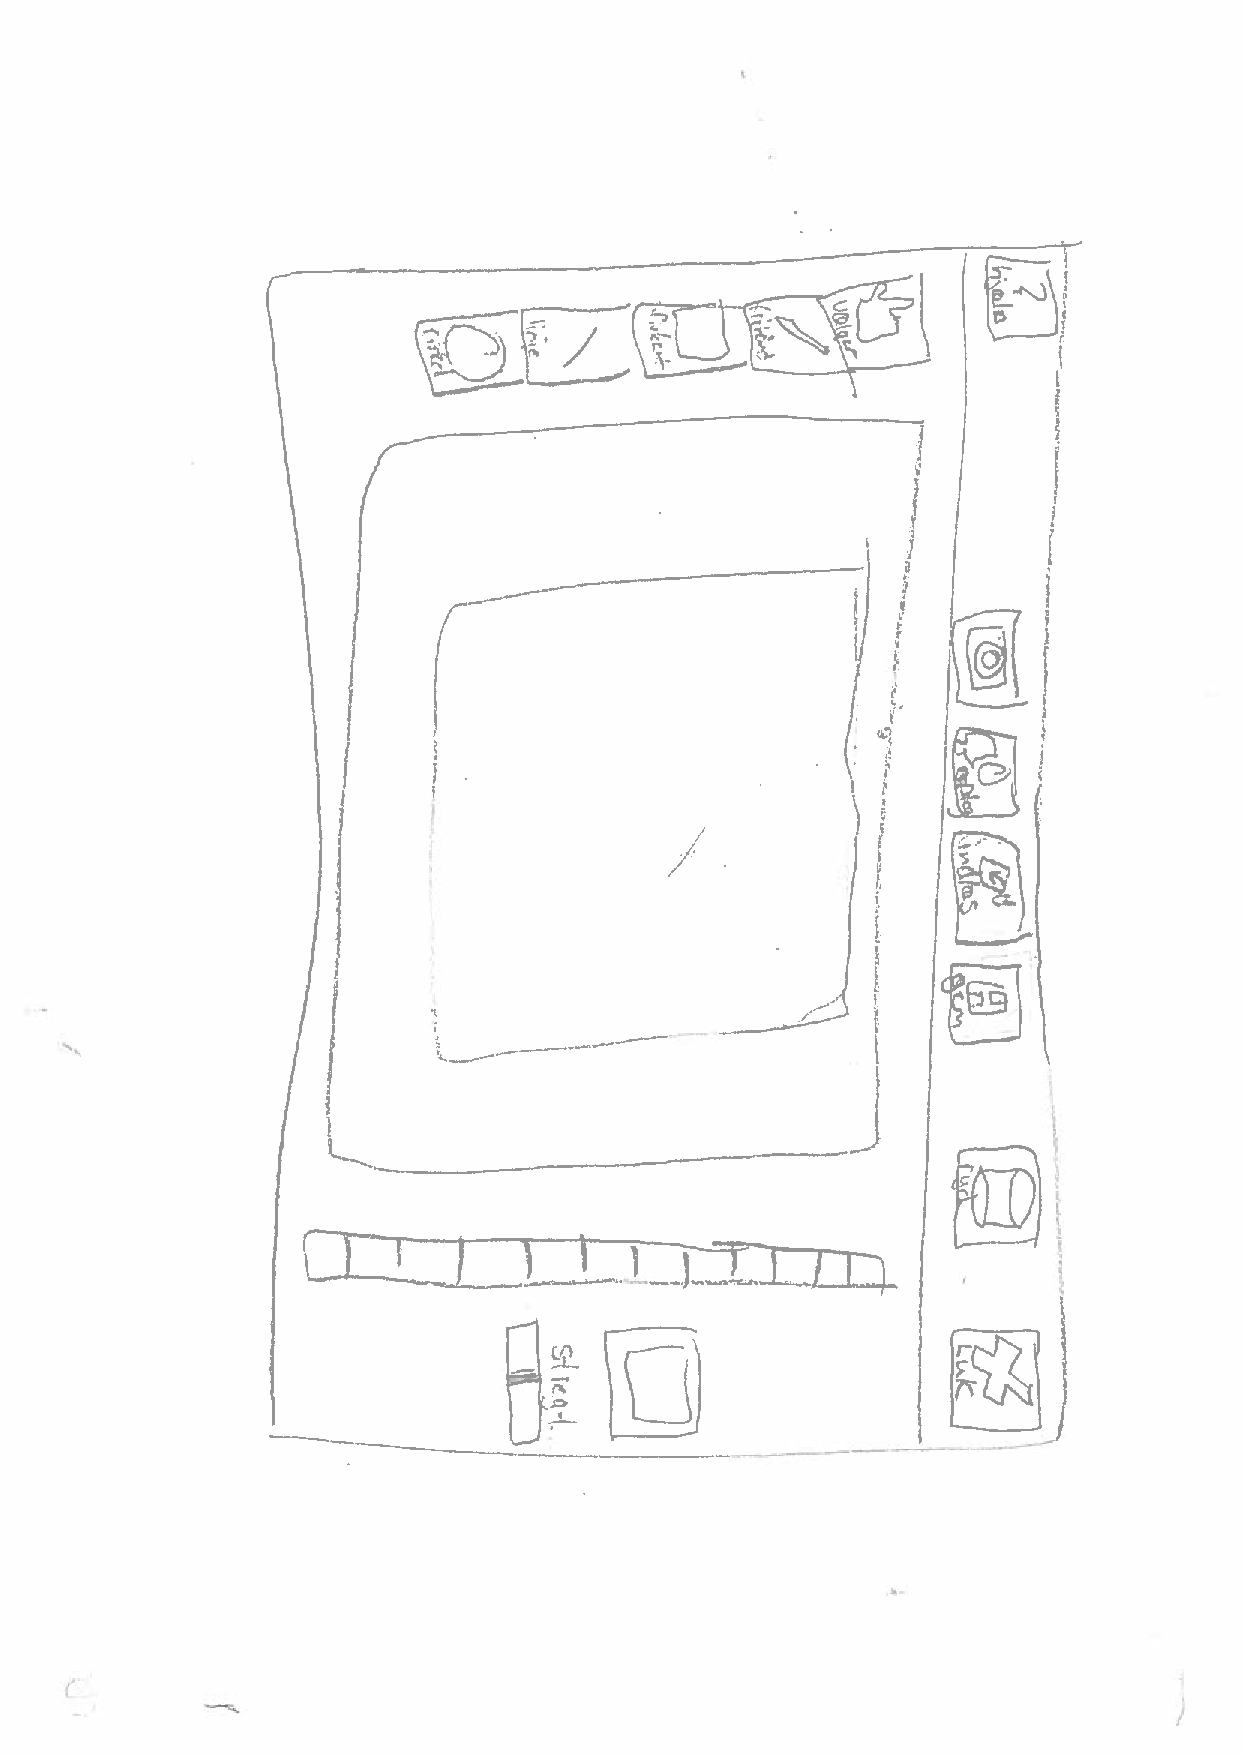
\includegraphics[angle=90, scale=0.5, trim = 4cm 5cm 2.5cm 4cm,clip]{sprint3/v2-drawfragment.pdf}
     \caption{Version 2 drawfragment.}
     \label{fig:v2drawfrag}
\end{figure}

Parts of the two prototypes were found satisfactory, and as of such a combination of the UI was performed.
It resulted in still having the separation of tools and their options, but making the \textit{drawFragment} being a more general layout, featuring the creation of pictograms instead of the drawing part solely.

\subsubsection*{Camera Dialogue}
The customers found it unintuitive to be able to take multiple pictures at a time and then later load some of the pictures for a pictogram.
For that reason, the camera dialogue should be changed to only be able to take one picture at a time.
When the picture is taken it can be verified, and then added to the pictogram, or discarded.

\begin{figure}[h]
     \centering
     \begin{subfigure}{0.45\textwidth}
          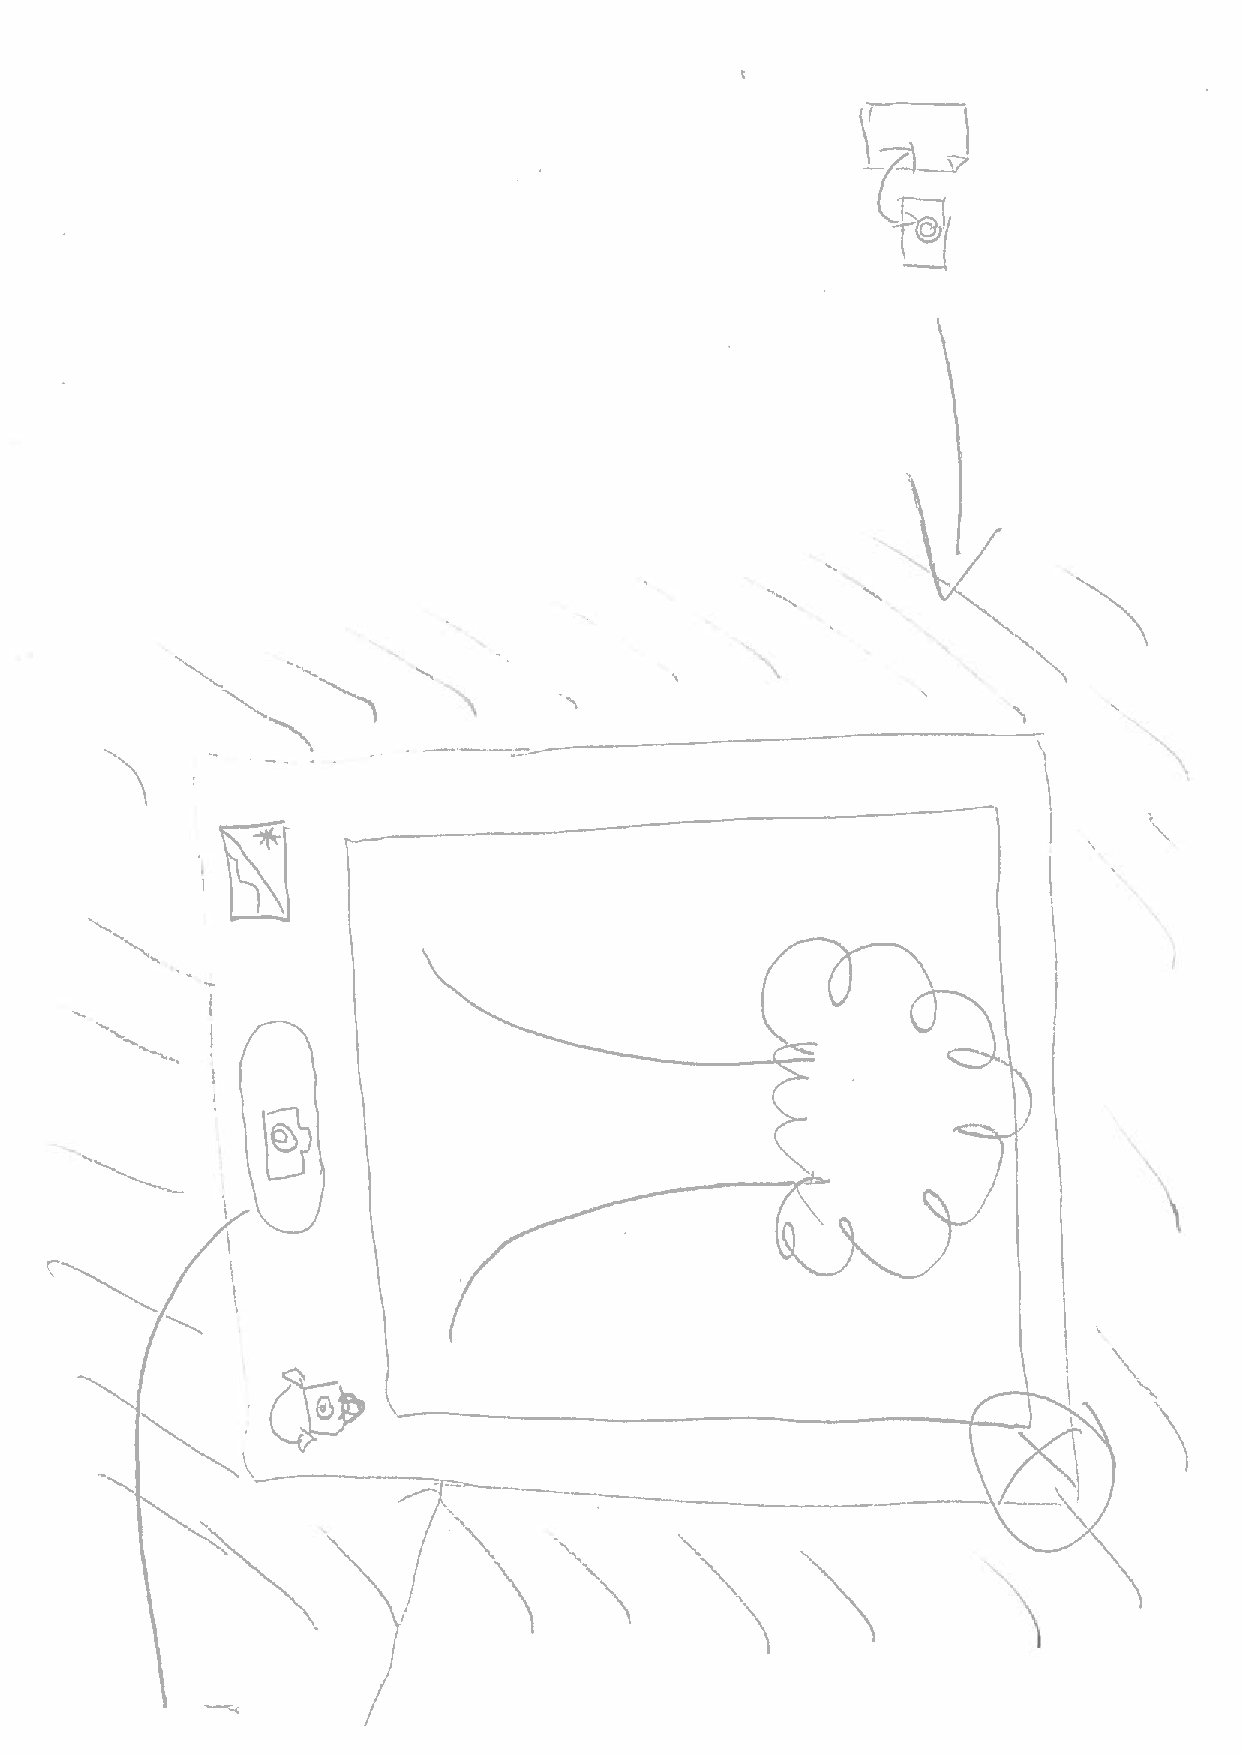
\includegraphics[angle=90, width = \textwidth, trim = 3cm 3cm 2.5cm 10cm,clip]{sprint3/camera-takepicture.pdf}
          \caption{Take Picture}
          \label{fig:cam-takepic}
     \end{subfigure}      
     \begin{subfigure}{0.45\textwidth}
          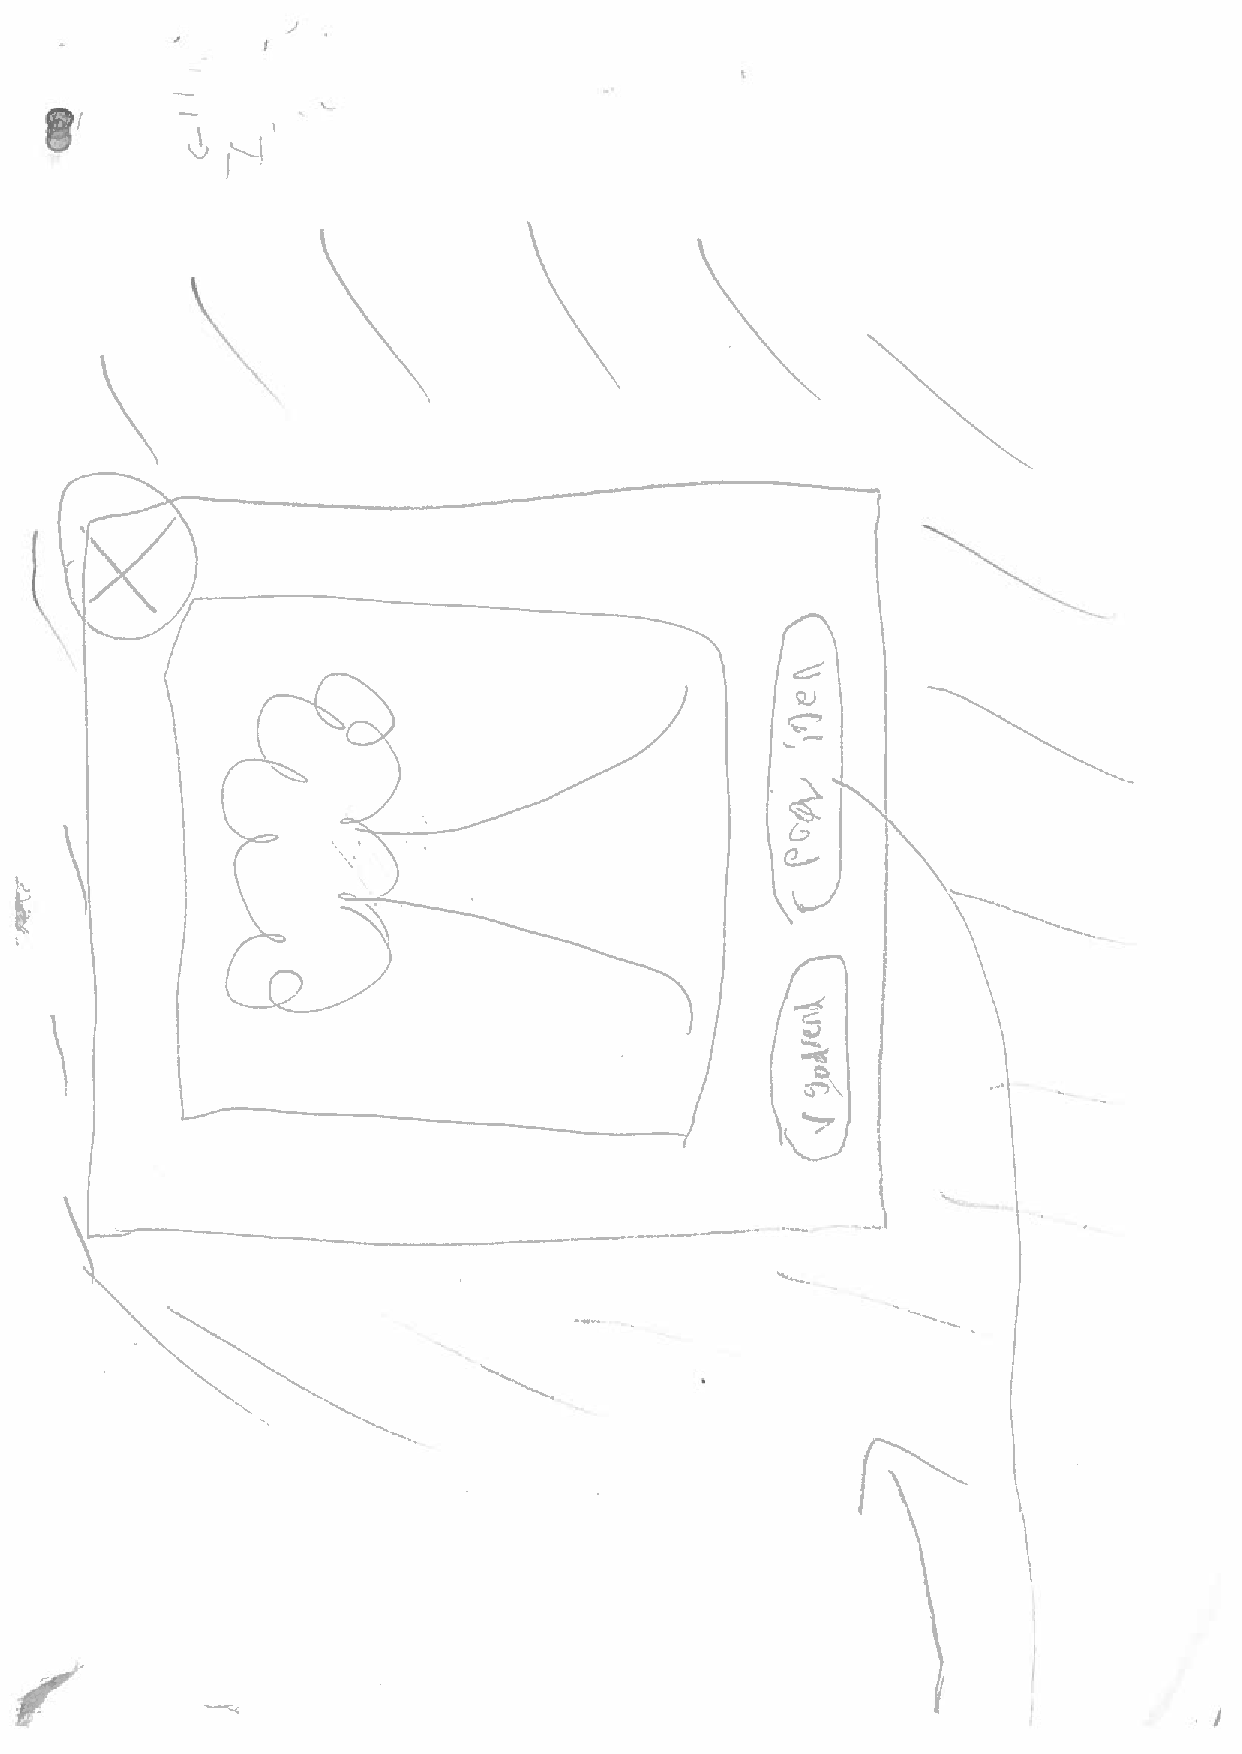
\includegraphics[angle=270, width = \textwidth, trim = 1cm 7cm 4.5cm 6.5cm,clip]{sprint3/camera-verify.pdf}
          \caption{Verify Picture}
          \label{fig:cam-verifypic}
     \end{subfigure}
     \caption{Camera Dialogue}
     \label{fig:cam-dialogue}
\end{figure}

\figref{fig:cam-dialogue} shows a prototype of the camera dialogue, where inspiration has come from popular image applications such as the inbuilt iOS camera and Instagram.\fxwarning{reference her.}
Seen in \figref{fig:cam-takepic} is the dialogue as it should look like when preparing to take a picture of a tree.
The button to the lower left is to swap between colour and black-white mode, which is a request of the customers.
In the lower right corner, a button to swap between front and back camera can be seen.
Finally, in the lower center, a button to take the picture can be seen.

When the picture is taken, you are transferred to the UI seen in \figref{fig:cam-verifypic}, where you have the option to accept the taken picture or to decline it, and return to the previous UI to take a new picture.

In the whole camera dialogue you always have the option to quit the dialogue by pressing the button in the upper right corner.
\subsection{Additional Work}\fxwarning{discuss this title, seems weird}
The implemented version of the UI is not tested yet, and as of such can not be determined as final yet.
Future sprints would have to focus on presenting the UI to the customers and perform usability tests to ensure that a good quality of the application is achieved.